\chapter{光晶格中系统的拓扑电子输运} \label{chap:chargepump}

本章,我们将讨论光晶格中拓扑物态的相关问题,着重讨论光晶格中的拓扑电子输运的话题。
首先,我们在 \ref{sec:adiabevolgeneral} 小节建立绝热演化的一般形式理论,给出周期性演化的绝热极限(\ref{sec:adiabatic} 节)下的条件,并针对单带情况(\ref{sec:adiab:single})和多带情况(\ref{sec:adiab:multi})分别推导出其绝热周期幺正演化的形式;对于前者,其绝热周期幺正演化带来 Berry 相角,而对于后者,其绝热周期幺正演化带来非阿贝尔 Berry 联络。这种情况下,不止对角元是重要的,非对角元也是重要的。
在第 \ref{sec:topocp} 节,我们将讨论周期绝热电子输运的问题,并讨论其与拓扑物态的关系;我们推导出在一维模型中,量子化的周期绝热电子输运与某种一维绕数(winding number)和二维陈数(Chern number)的等价关系,这也就是 Thouless 拓扑输运过程\cite{thouless1983};作为一个例子,我们将介绍 经典的 SSH 模型\cite{ssh1979}\footnote{与之类似的是 Majorana 的 Kitaev 链模型\cite{kitaev2001}},和基于该模型推广的 Rice-Mele 拓扑输运过程\cite{ricemele1982};该模型在光晶格中的实现在2013年由王磊老师等人提出\inlinecite{wanglei2013},并在2015-2016年由两个实验小组在超冷原子光晶格系统中实现\inlinecite{charge-pump-expr-2016-de,charge-pump-expr-2016-jp}。在 \ref{sec:creutz} 小节,我们介绍我们提出的 Creutz 梯\cite{creutz1999}上拓扑电子泵的模型\cite{creutz}。我们给出了该模型的完整的拓扑相图,并发现了一种新奇的拓扑输运过程,在这种过程中,电子的周期输运以偶数为单位,即,每个周期只能有2或者2的倍数的电荷被传输。这并不是简单的将周期乘以2——或简单的将模型进行双份备份——所导致的偶数为基数的拓扑输运过程,而是由模型的内禀性质所决定,区别于前面提到的 Rice-Mele 过程。对于这个发现,我们给出了解析的推导,和数值的检验。通过对含时薛定谔方程的演化进行数值模拟计算,我们发现在绝热极限下电子的输运过程确实具有完美的量子化平台;同时我们也计算了不满足绝热条件的情况下电子的输运过程,以进行对比。





\section{绝热演化通论}\label{sec:adiabevolgeneral}

对于一个量子力学系统,系统从一个初态开始的演化完全决定于以下引入的幺正演化算符\footnote{在本文中,省略的地方默认取自然单位 $\hbar=1$。}
\begin{align}
U(t_0,t)=\mathcal{T}e^{-\ii\int_{t_0}^t H(t')dt'}
\end{align}
这里 $\mathcal{T}$ 为时序算符,其精确的含义如下,
\begin{align}\label{def:unitary}
U(t_0, t)&=\mathcal{T}e^{-\ii\int_{t_0}^{t} H(t')dt'} \nonumber\\
&= \lim_{\mathclap{\substack{N\rightarrow\infty\\\Delta t\rightarrow0}}}\exp\Big[-\ii H(t_{N-1})\Delta t\Big]\exp\Big[-\ii H(t_{N-2})\Delta t\Big]\cdots\exp\Big[-\ii H(t_0)\Delta t\Big]\\
&= \lim_{\mathclap{\substack{N\rightarrow\infty\\\Delta t\rightarrow0}}}\prod_{j=0}^{N-1}\exp\Big[-\ii H(t_j)\Delta t\Big]
\end{align}
其中,
\begin{align}
t_{j} &= j\Delta t \\
N\Delta t &= t-t_0
\end{align}
对于静态(不含时)哈密顿量,
\begin{align}
H(t)\equiv H_0
\end{align}
因此有
\begin{align*}
U(t_0,t)=\exp[-\ii H_0(t-t_0)]
\end{align*}

若哈密顿量含时,则一般来说幺正演化算符不能做这样的简化,体系演化需通过上面的 (\ref{def:unitary}) 式进行一般的推演。然而对于一类特殊的含时体系,即周期含时的体系,其以周期为单位的幺正演化可以被继续简化。在这种情况下,有两个极限值得考虑:高频极限与绝热极限。前者是指,相比于体系的典型能量尺度,体系含时依赖的周期极短、频率极高,故称高频极限;而后者是指,相比于体系的典型能量尺度,体系含时依赖的周期极长、频率极低,体系“绝热”地处在每时每刻的瞬时本征态上,故称绝热极限。对于高频极限,这不是我们这一章关注的内容,将放到第 \ref{chap:floq} 章的第 \ref{sec:highfreq} 小节进行讨论。对于绝热极限,我们将在下面进行具体讨论,并把上面提到的“体系含时依赖的周期极长、频率极低,体系‘绝热’地处在每时每刻的瞬时本征态上”这句话进行定量刻画。

\subsection{绝热极限}\label{sec:adiabatic}
上面提到,绝热极限是指体系含时依赖周期极长的极限,这是相对于体系所处的典型能量尺度来说的,也就是说,在绝热极限下体系每时每刻都处在$H(t)$的瞬时本征态上。下面我们对这个条件进行具体的表述。
\footnote{以下推导可以参考众多经典的量子力学教科书,如\inlinecite{shankar,sakurai}。}

对于含时体系的哈密顿量 $H(t)$,在任意时刻 $t$,体系都有如下瞬时本征态
\begin{align}
H(t)|n(t)\rangle=E_n(t)|n(t)\rangle
\end{align}
$E_n$ 为瞬时本征态的本征能量。所有的 $\{|n(t)\rangle\}$ 构成了 $t$ 时刻体系的希尔伯特空间的一组完备基,体系的任何态的演化都可以用这组完备基来展开
\begin{align}\label{eq.psi}
|\psi(t)\rangle=\sum_na_n(t)e^{\ii\theta_n(t)}|n(t)\rangle
\end{align}
其中
\begin{align}
\theta_n(t)=(-1/\hbar)\int^tdt'E_n(t')
\end{align}
这里我们并没有指定规范,即每个 $|n(t)\rangle$ 的相角。但这并不影响绝热条件的推导,同样也不影响马上要提到的 Berry 相角。

考虑满足含时薛定谔方程的 $|\psi(t)\rangle$ ,
\begin{align}
\ii\hbar\partial_t|\psi(t)\rangle=H(t)|\psi(t)\rangle
\end{align}
将 (\ref{eq.psi}) 式带入可得,等式左边为
\begin{align}
\text{left} 
=& \ii\hbar\sum_n[(\dot{a}_n(t)+a_n(t)\ii\partial_t\theta_n(t))e^{\ii\theta_n(t)}+a_n(t)e^{\ii\theta_n(t)}\partial_t]|n(t)\rangle\\
=& \ii\hbar\sum_n\dot{a}_n(t)e^{\ii\theta_n(t)}|n(t)\rangle\\
    & +\sum_{n}E_n(t)a_n(t)e^{\ii\theta_n(t)}|n(t)\rangle\\
    & +\ii\hbar\sum_na_{n}(t)e^{\ii\theta_n(t)}\partial_t|n(t)\rangle
\end{align}
等式右边为
\begin{align}
\text{right} &= \sum_{n}E_n(t)a_n(t)e^{\ii\theta_n(t)}|n(t)\rangle
\end{align}
右边的项和左边的第二项消掉了,得到
\begin{align}
\sum_n\dot{a}_n(t)e^{\ii\theta_n(t)}|n(t)\rangle+a_{n}(t)e^{\ii\theta_n(t)}\partial_t|n(t)\rangle=0
\end{align}
将 $\langle m(t)|$ 从左边作用上去,得到
\begin{align}
\langle m(t)|\sum_n\dot{a}_n(t)e^{\ii\theta_n(t)}|n(t)\rangle+a_{n}(t)e^{\ii\theta_n(t)}\partial_t|n(t)\rangle=0
\end{align}
\begin{align}
\therefore \dot{a}_m(t)=-\sum_na_{n}(t)e^{\ii[\theta_n(t)-\theta_m(t)]}\langle m(t)|\partial_tn(t)\rangle
\end{align}
注意到,对于 $m\neq n$ 的情况,有
\begin{align}
\partial_t\langle m(t)|H(t)|n(t)\rangle
    &= \langle\partial_tm(t)|H(t)|n(t)\rangle \notag \\
    & \quad +\langle m(t)|\partial_tH(t)|n(t)\rangle \notag \\
    & \quad +\langle m(t)|H(t)|\partial_tn(t)\rangle\\
    &= -(E_n-E_m)\langle m(t)|\partial_tn(t)\rangle+\langle m(t)|\partial H/\partial t|n(t)\rangle
\end{align}
因此有,
\begin{align}
\langle m(t)|\partial_tn(t)\rangle=\dfrac{\langle m|\partial H/\partial t|n\rangle}{E_n-E_m}
\end{align}
因此,
\begin{align}
\dot{a}_m(t) &=-\sum_na_{n}(t)e^{\ii[\theta_n(t)-\theta_m(t)]}\langle m(t)|\partial_tn(t)\rangle\\
    &= -a_m(t)\langle m(t)|\partial_tm(t)\rangle-\sum_{n\neq m}a_{n}(t)e^{\ii[\theta_n(t)-\theta_m(t)]}\dfrac{\langle m(t)|\partial H/\partial t|n(t)\rangle}{E_n(t)-E_m(t)}
\end{align}

现在,假设我们从体系的第 $n$ 个本征态出发,即
\begin{align}
& a_n(0)=1\\
& a_{n'\neq n}(0)=0 \quad\text{(for $n\neq0$)}
\end{align}
那么,保留到一阶近似有
\footnote{零阶近似就是体系处在瞬时本征态上本身。}
\begin{align}\label{eq:amdot}
\dot{a}_m(t) 
    &= -a_{n}(t)\exp\left[-\dfrac{\ii}{\hbar}\int^tE_n(t')-E_m(t')dt'\right]\langle m(t)|\partial_tn(t)\rangle\\
    &= -a_{n}(t)\exp\left[-\dfrac{\ii}{\hbar}\int^tE_n(t')-E_m(t')dt'\right]\dfrac{\langle m(t)|\partial H/\partial t|n(t)\rangle}{E_n(t)-E_m(t)}
\end{align}
对此,绝热条件
\footnote{$\dot{a}_m$ 的量纲是 1/[时间],因此需要 $\hbar\dot{a}_m/\text{typical energy scale}\ll1$。而这里的典型能量尺度就是两个态的能量差,如基态到第一激发态,或两个能带的带隙。}
要求 $\dot{a}_m$ 非常小,
在绝热极限下趋于0,这样才能使得体系更趋于处在其瞬时本征态上。因此,由上两式引出绝热条件的两种表述:
\begin{itemize}
\item 第一种表述,\cite{niu2010}
\begin{align}\label{eq:am}
a_m(t)=-\dfrac{\langle m|\partial_t|n\rangle}{E_n-E_m}\ii\hbar\exp\left[-\dfrac{\ii}{\hbar}\int^tE_n(t')-E_m(t')dt'\right]
\end{align}
因此,
\begin{align}
-\dfrac{\langle m|\partial_t|n\rangle}{E_n-E_m}\ii\hbar\ll1
\end{align}
\item 第二种表述,\cite{sakurai}
\begin{align}
\dfrac{\langle m(t)|\partial H/\partial t|n(t)\rangle}{E_n(t)-E_m(t)}\equiv\dfrac{1}{\tau}\ll\langle m(t)|\partial_tm(t)\rangle\sim\dfrac{E_m}{\hbar}
\end{align}
\end{itemize}

对于固体材料来说,由于周期性晶格的存在,固体材料的色散关系形成能带。因此,根据上述绝热条件,对这样的周期性晶格体系来说,其绝热演化的条件被描述为:
\begin{itemize}
\item 考虑体系填充的能带的演化过程,该填充(一个或几个)能带与该(最高)能带之上的空带被有限大的带隙所分割(即,gapped system);
\item 体系的驱动频率极慢,以致于电子的激发过程很难发生。即,
\begin{align}
\hbar\omega \ll E_{\text{gap}}
\end{align}
这里 $\omega$ 是驱动频率,$E_{\text{gap}}$ 是满带和空带的带隙能量差。
\end{itemize}

下面分别考虑单带和多带的两种情况。



\subsection{单带模型}\label{sec:adiab:single}

首先,我们考虑单带模型的情况。考虑一个填充的基带,与之上的空带被有限大能隙所隔开。且随着时间演化,能隙不会关闭。考虑其绝热演化,即始终有 $\omega\ll E_{\text{gap}}$ 。则,其周期幺正演化算符为,
\begin{align}
U_n(T)&=\mathcal{T}e^{-\ii\int_{0}^T H(t')dt'}\\
&= \lim_{\mathclap{\substack{N\rightarrow\infty\\\Delta t\rightarrow0}}}\exp\Big[-\ii H(t_{N-1})\Delta t\Big]\exp\Big[-\ii H(t_{N-2})\Delta t\Big]\cdots\exp\Big[-\ii H(t_0)\Delta t\Big]\\
&= \lim_{\mathclap{\substack{N\rightarrow\infty\\\Delta t\rightarrow0}}}\exp\Big[-\ii H(t_{N-1})\Delta t\Big]|n(t_{N-1})\rangle\langle n(t_{N-1})|\exp\Big[-\ii H(t_{N-2})\Delta t\Big]|n(t_{N-2})\rangle\langle n(t_{N-2})|\cdots\\
&\qquad|n(t_{j+1})\rangle\uwave{\langle n(t_{j+1})|\exp\Big[-\ii H(t_j)\Delta t\Big]|n(t_{j})\rangle}\langle n(t_{j})|\cdots|n(t_{1})\rangle\langle n(t_{1})|\exp\Big[-\ii H(t_0)\Delta t\Big]
\end{align}
上式通过对(\ref{def:unitary})式的幺正演化算符指数插入一系列瞬时投影算符得到。其中被波浪线标注的部分展开来写为
\begin{align}
\langle n(t_{j+1})|\exp\Big[-\ii H(t_j)\Delta t\Big]|n(t_{j})\rangle
&= e^{-\ii E_n(t_j)\Delta t}\langle n(t_{j+1})|n(t_j)\rangle\\
&= e^{-\ii E_n(t_j)\Delta t}\bigg(\langle n(t_{j})|+\Delta t\dfrac{\partial\langle n(t_j)|}{\partial t}\bigg)|n(t_j)\rangle\\
&= e^{-\ii E_n(t_j)\Delta t}\bigg(1+\Delta t\langle\partial_t n(t_j)|n(t_j)\rangle\bigg)\\
&= e^{-\ii E_n(t_j)\Delta t}\bigg(1-\Delta t\langle n(t_j)|\partial_tn(t_j)\rangle\bigg)\\
&\rightarrow e^{-\ii E_n(t_j)\Delta t}\exp\bigg(-\Delta t\langle n(t_j)|\partial_tn(t_j)\rangle\bigg)
\end{align}
上式最后一行的极限取在
\begin{align}
N\rightarrow\infty, \quad\Delta t\rightarrow0
\end{align}
将其带回原式,可得
\begin{align}
U_n(T)&=\lim_{\mathclap{\substack{N\rightarrow\infty\\\Delta t\rightarrow0}}}|n(t_{N-1})\rangle e^{-\ii E_n(t_{N-1})\Delta t}e^{-\langle n(t_{N-1})|\partial_tn(t_{N-1})\rangle\Delta t}\cdots e^{-\ii E_n(t_0)\Delta t}e^{-\langle n(t_0)|\partial_tn(t_0)\rangle\Delta t}\langle n(t_0)|\\
&= \lim_{\mathclap{\substack{N\rightarrow\infty\\\Delta t\rightarrow0}}}\prod_{j=0}^{N-1}\exp\bigg[-\ii E_n(t_j)\Delta t\bigg]\exp\bigg[-\langle n(t_j)|\partial_tn(t_j)\rangle\Delta t\bigg]|n(t_{N-1})\rangle\langle n(t_0)|\\
&= \exp\bigg[-\int_0^T\langle n(t)|\partial_tn(t)\rangle dt\bigg]\exp\bigg[-\ii\int_0^TE_n(t)dt\bigg]|n(T)\rangle\langle n(0)|
\label{eq:ut-adiab-single-details}
\end{align}

事实上,由于模型的周期性的含时依赖,有
\begin{align}
H(t) = H(t+T)
\end{align}
因此
\begin{align}
|n(T)\rangle=|n(0)\rangle \quad (=|n\rangle)
\end{align}
$|n\rangle$ 为选定的某种规范。由此可看出,(\ref{eq:ut-adiab-single-details}) 式最后为 $|n\rangle$ 态的投影算符,而前面的两个因子中,第一项为 环路演化的 Berry 相角\cite{niu2010},第二项只是一个瞬时本征能量积分而来的幺正相因子。即,
\begin{align}
U_n(T) &= e^{\ii\gamma}e^{-\ii\int_0^TE_n(t)dt}|n\rangle\langle n|\\
\gamma &=\int_0^T\ii\langle n(t)|\partial_tn(t)\rangle dt
\end{align}
需要注意的是,Berry 相角与规范选取无关。
\footnote{事实上,从上式看出已经可以看出这点了。将 $|n(t)\rangle$ 换一个任意的规范,带进去结果不变。参考\inlinecite{niu2010}}

这样我们就得到了单带模型的绝热周期幺正演化。



\subsection{多带模型}\label{sec:adiab:multi}

对于更一般的情况,我们下面考虑多带模型。我们考虑 $l$ 个填充的能带上的体系的演化。对于这种情况,绝热条件要求最高的填充带之上有带隙,且驱动频率的能量尺度远小于带隙能量。

类似于单带情况下的推导,这里我们将 $\sum_n|n(t_j)\rangle\langle n(t_j)|$ 这一系列填充能带的瞬时投影算符插入 $U(T)$ 展开为  (\ref{def:unitary}) 式中的每个时间间隔中间。更一般的,我们计算如下矩阵元:
\begin{align}
[\mathscr{U}(t_{j+1},t_j)]_{mn}=&\langle m(t_{j+1})|\exp\Big[-\ii\Delta tH(t_j)\Big]|n(t_j)\rangle\\
=& \langle m(t_{j+1})|1-\ii\Delta tH(t_j)|n(t_j)\rangle\\
=& \langle m(t_{j+1})|n(t_j)\rangle-\ii\Delta t\langle m(t_{j+1})|H(t_j)|n(t_j)\rangle\\
=& \bigg[\langle m(t_j)|+\Delta t\langle\partial_tm(t_j)|\bigg]|n(t_j)\rangle\qquad 
\hdashrule[0.5ex]{4.2cm}{1pt}{1mm} \mathscr{U}_1\\
&\qquad-\ii\Delta t\bigg[\langle m(t_j)|+\Delta t\langle\partial_tm(t_j)|\bigg]|H(t_j)|n(t_j)\rangle \quad
\hdashrule[0.5ex]{1.7cm}{1pt}{1mm} \mathscr{U}_2
\end{align}
这里我们用到了
\begin{align}
|m(t_{j+1})\rangle=|m(t_j)\rangle+|\partial_tm(t_j)\rangle\Delta t
\end{align}
对虚线标注的两部分分别展开,有
\begin{align}
\mathscr{U}_1 &=\langle m(t_j)|n(t_j)\rangle+\Delta t\langle\partial_tm(t_j)|n(t_j)\rangle\\
&= \delta_{mn}-\Delta t\langle m(t_j)|\partial_tn(t_j)\rangle
\end{align}
和
\begin{align}
\mathscr{U}_2 &=-\ii\Delta t\bigg[\langle m(t_j)|+\Delta t\langle\partial_tm(t_j)|\bigg]|H(t_j)|n(t_j)\rangle\\
&= -\ii\Delta t\langle m(t_j)|H(t_j)|n(t_j)\rangle-\ii(\Delta t)^2\partial_tm(t_j)|H(t_j)|n(t_j)\rangle\\
&= -\ii\Delta tE_n(t_j)\delta_{mn}+\mathcal{O}(\Delta t^2)
\end{align}
因此,保留到 $\Delta t$ 的一阶,忽略更高阶\footnote{这对于一个自洽的推导是至关重要的。}的 $\mathcal{O}(\Delta t^2)$,我们得到
\begin{align}\label{eqn.umn}
[\mathscr{U}(t_{j+1},t_j)]_{mn}=\mathscr{U}_1+\mathscr{U}_2=\delta_{mn}-\ii\Delta t\bigg(\delta_{mn}E_{n}(t_j)-\ii\langle m(t_j)|\partial_tn(t_j)\rangle\bigg)
\end{align}

这部分事实上是矩阵
\begin{align}
\mathscr{U}(t_{j+1},t_j)=\sum_{m,n}\bigg|m(t_{j+1})\bigg\rangle \big[\mathscr{U}(t_{j+1},t_j)\big]_{mn} \bigg\langle n(t_j)\bigg|
\end{align}
从右向左依次作用。事实上,从 (\ref{eqn.umn}) 式可以清楚地看出,该矩阵可以被表示为
\begin{align}
[\mathscr{U}(t_{j+1},t_j)]_{mn}&=\mathscr{U}_1+\mathscr{U}_2=\delta_{mn}-\ii\Delta t\bigg(\delta_{mn}E_{n}(t_j)-\ii\langle m(t_j)|\partial_tn(t_j)\rangle\bigg)\\
&=\bigg(\mathbb{I}-\ii\Delta t\Big[\mathcal{E}(t_j)-\mathcal{A}(t_j)\Big]\bigg)_{mn}\\
&= \text{MExp}\bigg(-\ii\Delta t\Big[\mathcal{E}(t_j)-\mathcal{A}(t_j)\Big]\bigg)_{mn}
\end{align}
其中,
\begin{itemize}
\item $\text{MExp}$ 指的是矩阵的指数;
\item $\mathcal{E}(t_j)$ 是在 $t_j$ 时刻的瞬时哈密顿量对角化后的能量(对角矩阵);
\item $\mathcal{A}(t_j)$ 就是所谓的 定义在 $l$-带流形上的 \textit{非阿贝尔} Berry 联络,其矩阵元为 $\mathcal{A}_{mn}=\ii\langle m|\partial_tn\rangle$。
\end{itemize}

基于以上种种,得到多带情况下的周期幺正演化算符为
\begin{align}
U(t_f;t_0)=\mathcal{T}\exp\bigg(-\ii\int_{t_0}^{t_f}\mathcal{E}(t)-\mathcal{A}(t)dt\bigg)
\end{align}
这在能量瞬时本征态的基矢下写为 $l\times l$ 的矩阵。注意到,$\mathcal{E}(t)$ 总是对角的,而对于一个周期的演化(loop),有 $t_f-t_0=T$,
\begin{align}
U(T)=\mathcal{T}\exp\bigg(-\ii\int_{0}^{T}\mathcal{E}(t)-\mathcal{A}(t)dt\bigg)
\end{align}
可以看出,演化算符的形式,在能量瞬时本征态的基矢下,能量的信息仅包含在对角元中,而非阿贝尔 Berry 联络的信息既包含在对角元中,也包含在非对角元中。相比于单带模型绝热周期幺正演化简单为一个数,和考虑平衡态一类问题时仅仅对矩阵求迹,对于多带模型下的绝热幺正周期演化,非对角元信息是非平庸的,不能被丢掉。






\section{绝热周期电子输运与拓扑物态}\label{sec:topocp}
对于晶格中的某一个能带,$\vect{q}$准动量的流密度由下式给出
\begin{align}
j(\vect{q}, t) &= \left\langle u(\vect{q}, t)\left|\dfrac{\partial H(\vect{q}, t)}{\partial\vect{q}} \right|u(\vect{q}, t)\right\rangle
% &= \dfrac{\partial \mathcal{E}(\vect{q}, t)}{\partial\vect{q}} 
% - \left\langle u(\vect{q}, t)\left|\partial/\partial_{\vect{q}}\right|u(\vect{q}, t)\right\rangle
\end{align}
利用 (\ref{eq:amdot}) 式 和 (\ref{eq:am}) 式,将上式中 的右矢 $|u(\vect{q}, t)\rangle$ 进行替换,可得
\begin{align}
j(\vect{q}, t)
&= \langle u(\vect{q},t)|\partial H(\vect{q},t)/\partial\vect{q}|u(\vect{q},t)\rangle \\
&= \langle u|\left(\partial_{\vect{q}} H\right) \left(-\ii\sum_{u\neq u'}\dfrac{|u'\rangle\langle u'|\partial_t u\rangle}{E_u - E_u'}\right) \\
&= \dfrac{\partial E_u}{\partial\vect{q}} - \ii\left[\left\langle\dfrac{\partial u}{\partial \vect{q}}\bigg|\dfrac{\partial u}{\partial t}\right\rangle - \left\langle\dfrac{\partial u}{\partial t}\bigg|\dfrac{\partial u}{\partial \vect{q}}\right\rangle\right]
\end{align}
因此,总的流为
\begin{align}
j(t) = \int_{\text{BZ}}\left(\frac{d\vect{q}}{2\pi}\right)^{d} j(\vect{q}, t)
\end{align}
其中 $d$ 为晶格维度。因此,体系在一个周期内的电子输运为
\begin{align}
\Delta n = \int_0^Tj(t)dt
\end{align}
对于一维晶格,将上式写开,
% \begin{align}
% \Delta n &= \int_0^Tj(t)dt \\
% & = - \frac{1}{2\pi}\int_0^T\int_{\text{BZ}}dtdq \left\langle u(\vect{q}, t)\left|\partial/\partial_{\vect{q}}\right|u(\vect{q}, t)\right\rangle \\
% & = \frac{1}{2\pi}\int_0^T\int_{\text{BZ}}dtdq \ii\cdot\ii \left\langle u(\vect{q}, t)\left|\partial/\partial_{\vect{q}}\right|u(\vect{q}, t)\right\rangle \\
% & = \frac{1}{2\pi}\int_0^T\int_{\text{BZ}}dtdq \ii\left[\left\langle\dfrac{\partial u(\vect{q},t)}{\partial t}\bigg|\dfrac{\partial u(\vect{q},t)}{\partial\vect{q}}\right\rangle - \left\langle\dfrac{\partial u(\vect{q},t)}{\partial\vect{q}}\bigg|\dfrac{\partial u(\vect{q},t)}{\partial t}\right\rangle\right] \\ 
% & = \frac{1}{2\pi}\int_0^T\int_{\text{BZ}}dtdq F_{\vect{q}t}\label{Chern}
% \end{align}
\begin{align}
n &= \int_0^Tj(t)dt \\
& = \frac{1}{2\pi}\int_0^T\int_{\text{BZ}}dtdq \ii\left[\left\langle\dfrac{\partial u(\vect{q},t)}{\partial t}\bigg|\dfrac{\partial u(\vect{q},t)}{\partial\vect{q}}\right\rangle - \left\langle\dfrac{\partial u(\vect{q},t)}{\partial\vect{q}}\bigg|\dfrac{\partial u(\vect{q},t)}{\partial t}\right\rangle\right] \\ 
& = \frac{1}{2\pi}\int_0^T\int_{\text{BZ}}dtdq F_{\vect{q}t}\label{Chern}
\end{align}
这里,$F_{\mu\nu}$ 是二维参数空间的 Berry 曲率,此处参数空间即 $(\vect{q}, t)$ 空间。上面最后一行实际上给出了以 $(\vect{q}, t)$ 为参数空间的 Berry 曲率在全空间的积分,称为陈数(Chern number)。\footnote{二维材料 Chern 数算法详见附录} 注意到参数空间的拓扑结构为 Torus($T^2$),事实上对于二维体系该积分刻画了一个从 参数空间的Torus 向球面($S^2$)的映射,因此这个积分后的常数为整数。


因此,上述一维晶格上的绝热电子输运过程实际上跟二维拓扑材料的刻画有着密切关系,其一个周期的电子输运等于将时间 $t$ 延展为一个参数方向的二维材料的 Chern 数。这个数是一个量子化的整数,因此上述过程也称为拓扑电子输运。值得注意的是,在以上简化版的推导中,绝热极限的条件已经隐含在里面,更具体和详细的讨论见 David J. Thouless 1983 年的文章\inlinecite{thouless1983}。此外,上述电子输运与Chern数的关系还有另一种推导方式是利用能带上波函数的极化(Polarization)来推导,可参考\inlinecite{topobook} 和 \inlinecite{resta1994}。

另一个值得注意的事实是,上述一维晶格的绝热演化过程也可以联系到一维材料的拓扑数上。一个用来刻画一维材料的拓扑数是绕数(winding number),简单来说就是一个 U(1) 的参数空间到另一个\textit{不能收缩的} U(1) 参数空间的映射\footnote{这种刻画与数学中的同伦群有关}。这里一维绕数被引入为\cite{kitagawa2010,topoclassify2016}
\begin{align}
\nu_1=\dfrac{1}{2\pi}\int_{-\pi}^{\pi}dq Tr[U_q(T)^{-1}\ii\partial_qU_q(T)]\label{wind}
\end{align}
下面我们来推导其与绝热电子输运的关系。注意到,在绝热极限下,上一节我们得到
\begin{align}
U_n(q,T) &= e^{\ii\gamma(q)}e^{-\ii\int_0^TE_n(q,t)dt}|n\rangle\langle n|
\end{align}
其中
\begin{align}
\gamma(q) &=\int_0^T\ii\langle n(q,t)|\partial_tn(q,t)\rangle dt
\end{align}
因此,
\begin{align}
U(q,T)^{-1}\ii\partial_qU(q,T)=-\partial_q\gamma(q)+\int_0^T\partial_qE_n(q,t)dt
\end{align}
因此可得,
\begin{align}
\nu_1^{(n)}&= \dfrac{1}{2\pi}\int_{-\pi}^{\pi}dq U_n(q,T)^{-1}\ii\partial_qU_n(q,T)\\
&= -\dfrac{1}{2\pi}\gamma(q)\bigg|_{-\pi}^{\pi}\\
&= \dfrac{1}{2\pi}\int_{-\pi}^{\pi}dq\int_0^Tdt\;\ii\bigg[\langle\partial_qn(q,t)|\partial_tn(q,t)\rangle-\langle\partial_tn(q,t)|\partial_qn(q,t)\rangle\bigg]
\end{align}
这就证明了绝热周期电子输运等于上述定义的绕数。

类似的,我们还可以考虑高维的电子输运过程和高维的拓扑数,例如,如下的三维绕数
\begin{align}
\nu_3=\int\dfrac{d^3q}{24\pi}\varepsilon^{\alpha\beta\gamma}Tr[(U_{\vect{q}}^{-1}\partial_{\vect{q_{\alpha}}}U_{\vect{q}})(U_{\vect{k}}^{-1}\partial_{\vect{q_{\beta}}}U_{\vect{q}})(U_{\vect{q}}^{-1}\partial_{\vect{q_{\gamma}}}U_{\vect{q}})]
\end{align}
以及最近的四维量子霍尔效应与二维电子输运的实验\cite{4dqhall-expr-2018}。


\subsection{SSH模型 和 Rice-Mele 类型的拓扑电子输运}\label{sec:ssh}

我们对众所周知的 SSH 模型\cite{ssh1979}(与 Kitaev 链模型\cite{kitaev2001}类似)讨论由其推广的 Rice-Mele 模型上的拓扑电子输运过程。

SSH 模型哈密顿量写作
\begin{align}
H(t) &=\sum_j-(J+\delta)a_j^{\dagger}b_j-(J-\delta)a_{j+1}^{\dagger}b_j+h.c.
\end{align}
该模型具有手征对称性\footnote{见\ref{sec:dynsymm}节介绍的二分晶格手征变换},能谱上下对称。除了 $\delta=0$ 的情况,该模型均为有能隙(gapped)模型\footnote{Peierls instability makes it not easy to stay gapless.}
该模型属于拓扑分类\cite{topoclassify2016}中的 AIII 类,该类在后面第 \ref{sec:topoml} 章还会讲到。在傅立叶变换到 $q$-空间后,该两能带模型的哈密顿量具有$\sigma_x$,$\sigma_y$ 项,没有 $\sigma_z$ 项(这也是其手征对称性的来源), 且在特定构型的开边界条件下有局域的边界态,对此 Kitaev 给出了其波函数的严格解析解\cite{kitaev2001}。

Rice-Mele 模型的哈密顿量写作
\begin{align}
H(t) &=\sum_j-(J+\delta)a_j^{\dagger}b_j-(J-\delta)a_{j+1}^{\dagger}b_j+h.c.+\Delta(a_j^{\dagger}a_j-b_j^{\dagger}b_j)
\end{align}
比起 SSH 模型,Rice-Mele 模型的区别是添加了二分的局域化学势项。该项的添加对于电荷输运来说至关重要。简单来说,由于该项的添加,其 $q$-空间哈密顿量将一般地具有 $\sigma_x$,$\sigma_y$,$\sigma_z$ 三个分量,因此可能有非零 Chern 数。而根据上一节推导,非零 Chern 数意味着量子化的周期性绝热电荷输运。具体来说,傅立叶变换到 $q$-空间的哈密顿量写作,

\begin{align}
\mathcal{H}(q)
&=-2J\cos(\frac{qa}{2})\sigma_x-2\delta\sin(\frac{qa}{2})\sigma_y+\Delta\sigma_z
\end{align}

现在我们来考虑含时演化问题。例如,引入如下的含时依赖,
\begin{align}
H(t) &=\sum_j-(J+\delta\sin(\omega t))a_j^{\dagger}b_j-(J-\delta\sin(\omega t))a_{j+1}^{\dagger}b_j+h.c.+\Delta\cos(\omega t)(a_j^{\dagger}a_j-b_j^{\dagger}b_j)
\end{align}
则在 $q$-空间有
\begin{align}
\mathcal{H}(q,t)
&=-2J\cos(\frac{qa}{2})\sigma_x-2\delta\sin(\omega t)\sin(\frac{qa}{2})\sigma_y+\Delta\cos(\omega t)\sigma_z
\end{align}
容易计算\footnote{参见附录\ref{sec:chern}章},该模型 $(q,t)$ 空间 Chern 数为$\pm 1$。\footnote{上下两个band分别为+1,-1,或反之,依赖于定义。} 因此,该模型下应该有周期性的绝热拓扑电子输运。对此,在实验\inlinecite{charge-pump-expr-2016-de,charge-pump-expr-2016-jp}中有所验证,通过利用光晶格对Rice-Mele模型进行量子模拟,确实看到了冷原子气体云的周期性量子化的输运。

\begin{figure}[!htb]
\centering
\begin{subfigure}{.48\textwidth}
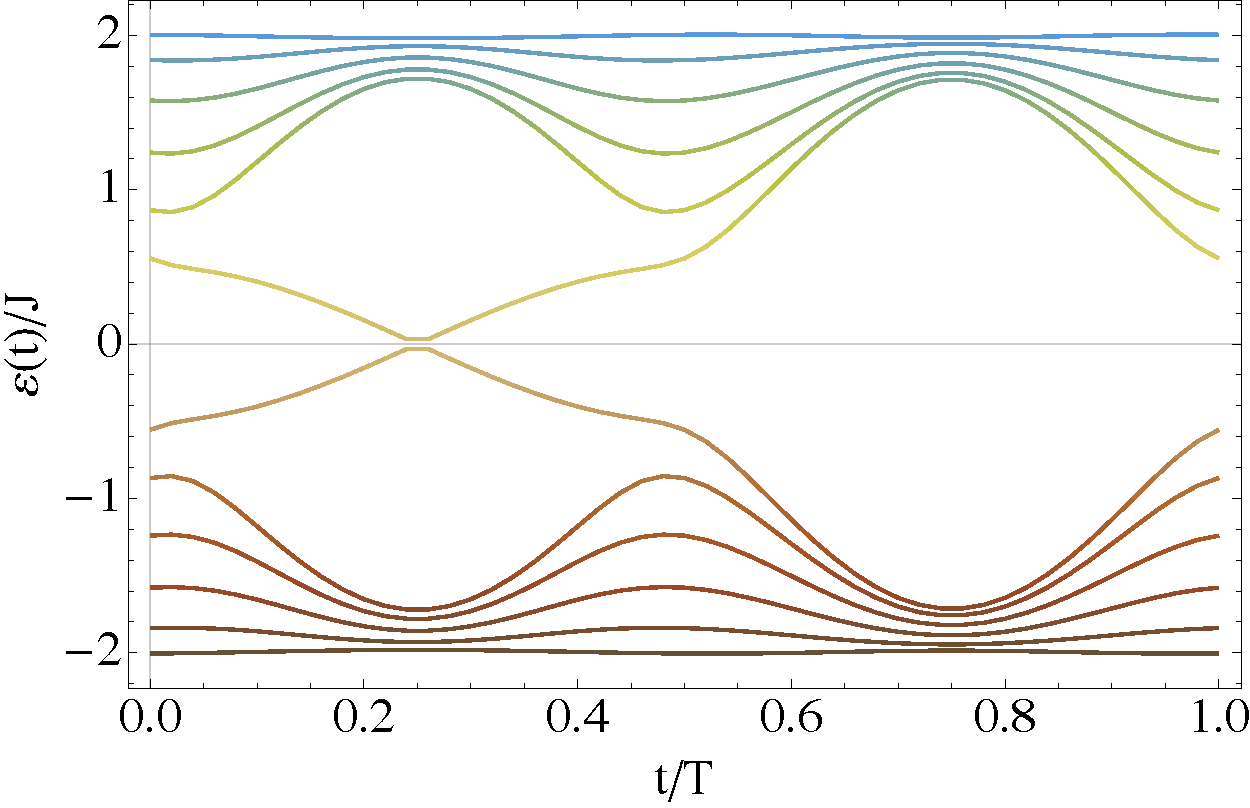
\includegraphics[width=1.\columnwidth]{chap2_topo/rmte_obc_12}
\end{subfigure}
\begin{subfigure}{.48\textwidth}
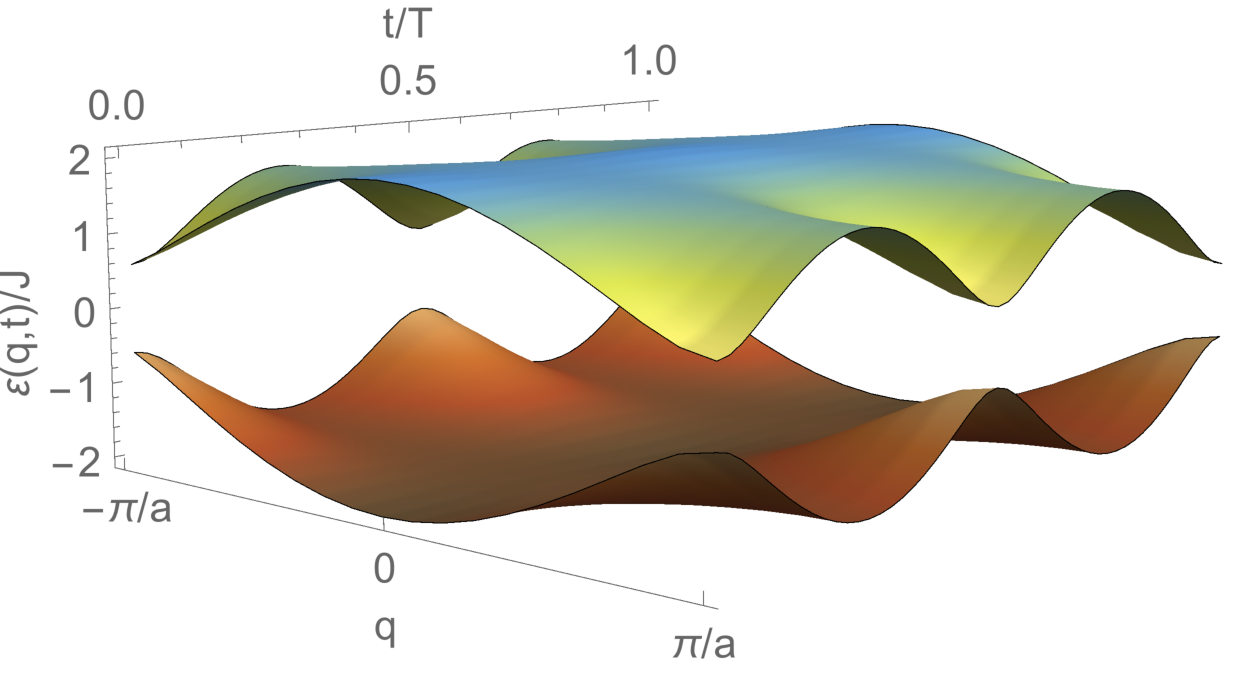
\includegraphics[width=1.\columnwidth]{chap2_topo/rmte_pbc_1}
\end{subfigure}
\caption{Rice-Mele 模型一个典型的非平凡路径演化下开边界条件、周期性边界条件下的能谱。(左)12个格点的开边界条件;(右)周期性边界条件。模型参数:$\delta/J=-0.85$, $\Delta/J=0.5$。}
\label{fig:rmterg}
\end{figure}
对该模型我们画出其沿非平凡路径演化下,分别在开边界条件、周期性边界条件下的能谱,见图 \ref{fig:rmterg} 所示。
从图 \ref{fig:rmterg} (左)可看到,能带中有边界态的存在\footnote{根据 Bulk Edge Correspondence,这也是应该的。}。它们沿着开放的边界\footnote{在此处,时间维度取为周期性,开放的维度即是一维晶格的维度}手征地运动,这就是电荷输运(Charge Pumping)的过程。
\footnote{这样就是经典的 Laughlin's Gauge Argument 所说的事情,可参考\inlinecite{laughlin1981}。这篇文献是作者早期接触到的最经典的几篇文献之一,短小精悍,论述和计算都很简单,但极度不平凡。Laughlin 用非常简单的计算展示了 Quantum Hall 体系中最不平庸的事实,其物理根源与 TKNN 等是一样的。虽然 Laughlin 所讨论的是 Quantum Hall 体系,但实际上和作者这儿演示的是同一回事。所有的 Topological Charge Pumping 本质上都是一样的,都是 twisted boundary conditions。}


\begin{figure}[!htb]
\centering
\begin{subfigure}{.4\textwidth}
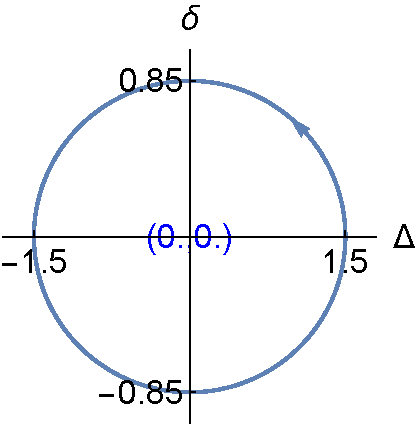
\includegraphics[width=1.\columnwidth]{chap2_topo/tRM_6_evol}
\end{subfigure}
\begin{subfigure}{.55\textwidth}
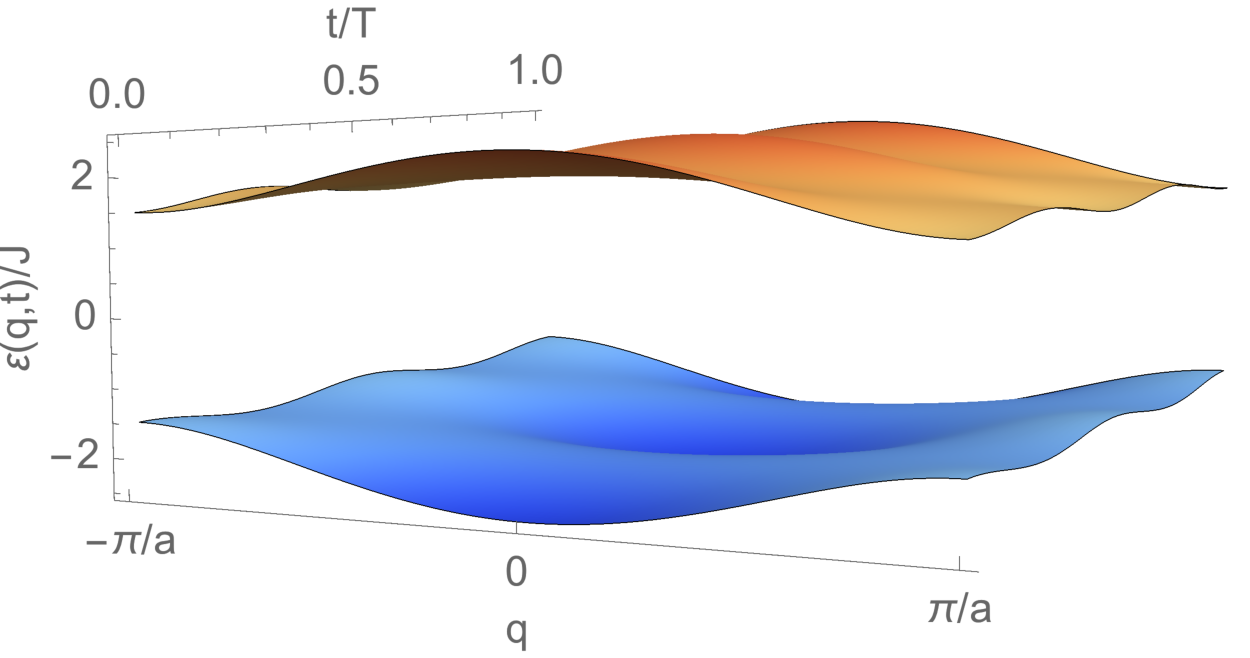
\includegraphics[width=1.\columnwidth]{chap2_topo/tRM_6_eqt}
\end{subfigure}\\
\begin{subfigure}{.45\textwidth}
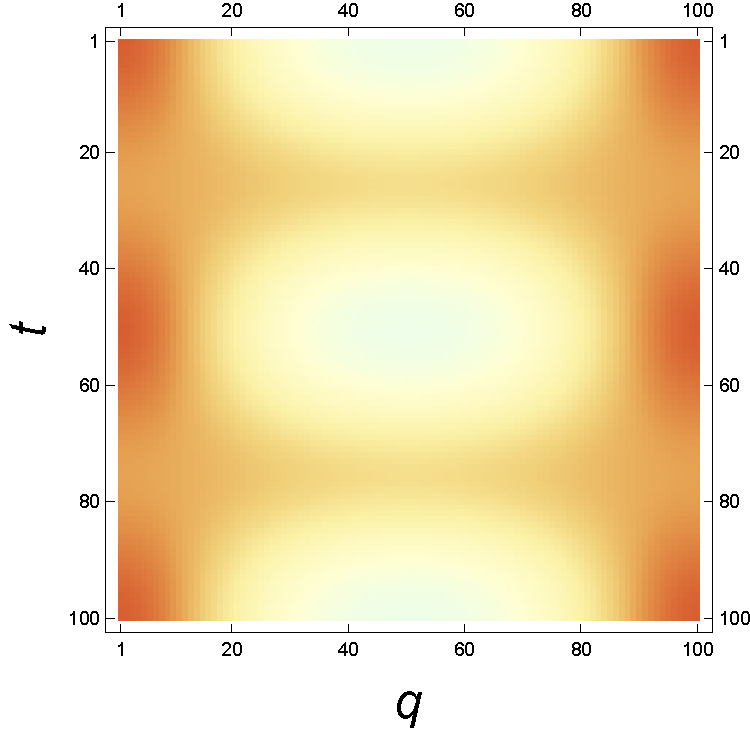
\includegraphics[width=1.\columnwidth]{chap2_topo/tRM_6_bf1}
\end{subfigure}
\begin{subfigure}{.45\textwidth}
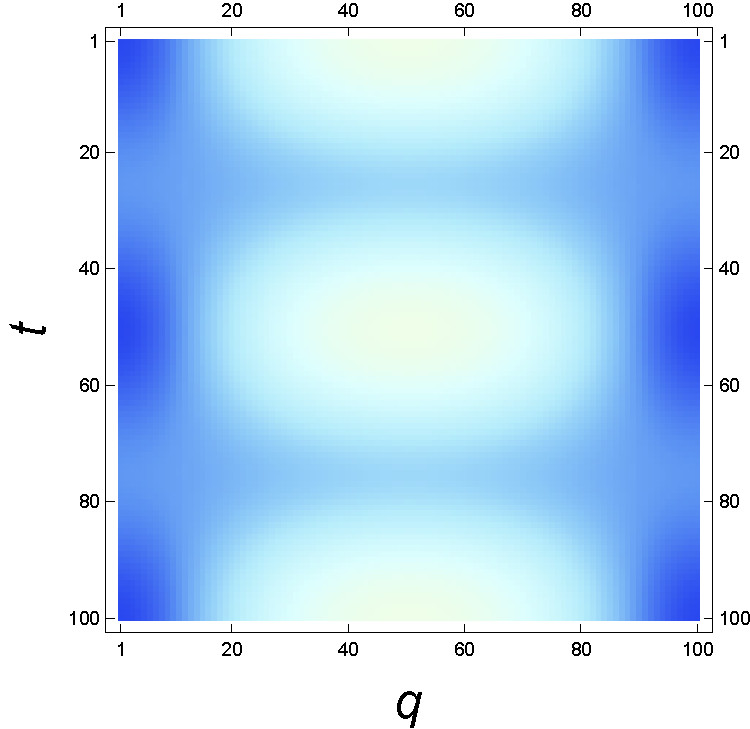
\includegraphics[width=1.\columnwidth]{chap2_topo/tRM_6_bf2}
\end{subfigure}
\caption{Rice-Mele 一个典型的非平庸路径。上栏:左为路径在 $(\delta, \Delta)$-参数空间的示意图,右为能带结构。下栏:上下两个能带的 Berry 曲率场。模型参数:$\delta/J=-0.85$, $\Delta/J=1.5$。}
\label{fig:rmtberry}
\end{figure}

我们还对一个代表性的非平凡的演化路径计算了上下两个能带的离散化到 $100\times100$ 的 Berry 曲率场,参见图 \ref{fig:rmtberry} 所示。其积分之后就是两个能带的 Chern 数,分别得 $\pm1$。

Rice-Mele 非平凡拓扑电子输运在光晶格中的实现在由王磊老师等人于2013年提出\inlinecite{wanglei2013},并在随后由两个实验小组在超冷原子光晶格系统中实现\inlinecite{charge-pump-expr-2016-de,charge-pump-expr-2016-jp}。





\section{ Creutz 梯上的拓扑电子泵}\label{sec:creutz}
这一节我们介绍我们在 Creutz 梯上提出的拓扑电子泵。Creutz 梯的模型由 Michael Creutz 于 1999 年在\inlinecite{creutz1999}文章中提出,旨在研究格点规范理论。原始的 Creutz 模型哈密顿量写作
\begin{align}
\hat{H} =&-\sum_{j} [J_X e^{\ii\theta} \hat{a}_{j+1}^\dag \hat{a}_{j}+J_X e^{-\ii\theta} \hat{b}_{j+1}^\dag \hat{b}_{j} + J_Y \hat{a}_j^\dag \hat{b}_j 
\nonumber\\
&+ J_D \hat{a}_j^\dag \hat{b}_{j+1}+J_D \hat{b}_j^\dag \hat{a}_{j+1} +\textrm{H.c.}]
\end{align}
该模型在特定参数下存在局域化的解,由于 Peierls 相角干涉的原因,局域化在某一对(纵向)格点上的粒子无法跃迁到其他格点\cite{creutz1999}。这让我们联想到 SSH 上类似的情况:SSH 模型中,特定参数下局域化的边界态波函数,当 $J_{\text{out}}\ll J_{\text{in}}$ 时,边界态波函数向体态里延伸的成分非常少(见 \inlinecite{kitaev2001} 中给出的解析解),当极端情况下 $J_{\text{out}}=0$, $J_{\text{in}}=1$ 时,波函数完全局域化在(最外的,或内部的一对)格点上,无法传播。这启发我们,在 Creutz 模型中也可能存在非平庸的拓扑电子输运的过程。

我们提出以下推广的 Creutz 模型。模型哈密顿量写作,
\begin{align}
\hat{H} =&-\sum_{j} [J_X e^{\ii\theta} \hat{a}_{j+1}^\dag \hat{a}_{j}+J_X e^{-\ii\theta} \hat{b}_{j+1}^\dag \hat{b}_{j} + J_Y e^{-\ii\phi} \hat{a}_j^\dag \hat{b}_j 
\nonumber\\
&+ J_D \hat{a}_j^\dag \hat{b}_{j+1}+J_D \hat{b}_j^\dag \hat{a}_{j+1} +\textrm{H.c.}]
\end{align}
与原始 Creutz 哈密顿量的区别在于在 $J_Y$ 跃迁上加了 $e^{-\ii\phi}$ 的相角。
如图 \ref{fig:creutz:schematic} 所示,图 \ref{fig:creutz:schematic} (a) 为 Creutz 梯的示意图。
\begin{figure}[!htb]
\centering
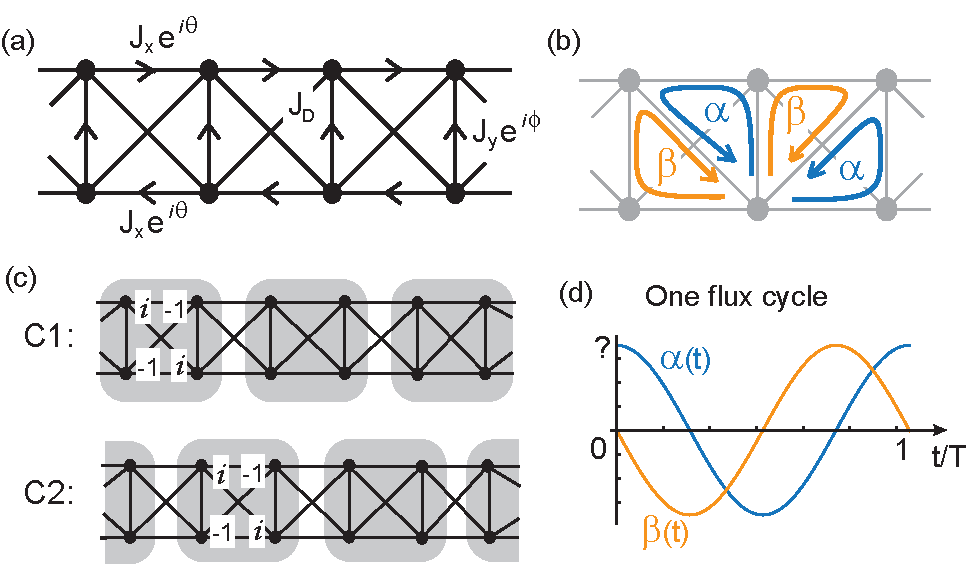
\includegraphics[width=1.\columnwidth]{creutz/fig1}
\caption{Creutz 模型示意图。(a) Creutz 梯晶格模型示意图,该模型由两个 Peierls 相角,单腿上跃迁 $J_Xe^{\ii\theta}$ 中的 $\theta$ 和相邻腿之间跃迁 $J_Ye^{-\ii\phi}$ 中的 $\phi$;(b) 该模型的两个相角也等价于用图示的 $\alpha$, $\beta$ 来刻画;(c) 对于该模型,在特定参数下有局域在方块(plaquette)上的局域态,由于干涉的原因,其不能跃迁到其他格点或方块上\cite{creutz,creutz1999};这种由干涉原因所导致的局域化波函数有两种构型,即图中的 $C_1$ 和 $C_2$,类比于 SSH 模型中调节 $J_1$, $J_2$ 时的两种局域化构型;(d) $\alpha$, $\beta$ 的一种典型的含时依赖周期。(取自\inlinecite{creutz})}
\label{fig:creutz:schematic}
\end{figure}
变换到 $k$-空间,哈密顿量写作
\begin{align}
H(k)=-\begin{pmatrix} 2 J_X \cos(ka-\theta)& 2 J_D\cos(ka)+J_Y e^{-\ii\phi}\\
2 J_D\cos(ka)+J_Y e^{\ii\phi}& 2 J_X \cos(ka+\theta)\end{pmatrix}
\end{align}
以上哈密顿量的一般形式具有 $\sigma_x$, $\sigma_y$, $\sigma_z$ 三个分量,可以预期参数空间存在非平凡的路径,使得扩展的 $(k,t)$-二维参数空间具有非零 Chern 数,这也意味着找到这样的参数路径并使之具有时间依赖,将有非平凡的托普电子输运过程。意即,这种情况下由 $(k,t)$ 向球面的映射能\textit{同向}覆盖一次或几次球面。而根据上一节的结论,非零 Chern 数意味着其周期性绝热电子输运过程的拓扑非平庸。

事实上,我们可以对上述模型的拓扑结构进行全面的分析。对于一维模型,一个可以用来刻画其拓扑结构的量是 Zak 相角\cite{zak1989},这实际上是一种能带中的 Berry 相角。Zak 相角本身并不特殊,但选定规范后,Zak 相角的差是一个绝对的数,可以用来区分平庸和非平庸的物态和过程。这方面的实验见\inlinecite{zak-expr-2013}。对于该 Creutz 梯模型,我们给出其参数空间的完整相图,见图 \ref{fig:creutz:topophase} 所示。参数空间中的实线和虚线代表相边界的地方,也就是体系发生简并的地方。因此这些线也叫简并线(degeneracy lines)。在参数空间中穿过实线或虚线时,体系的能隙会关闭再打开,并且发生能带反转(band inversion)\cite{topobook}。围绕这样的简并线形成的参数环路,其含时依赖可以给出拓扑电子输运的行为。
\begin{figure}[!htb]
\centering
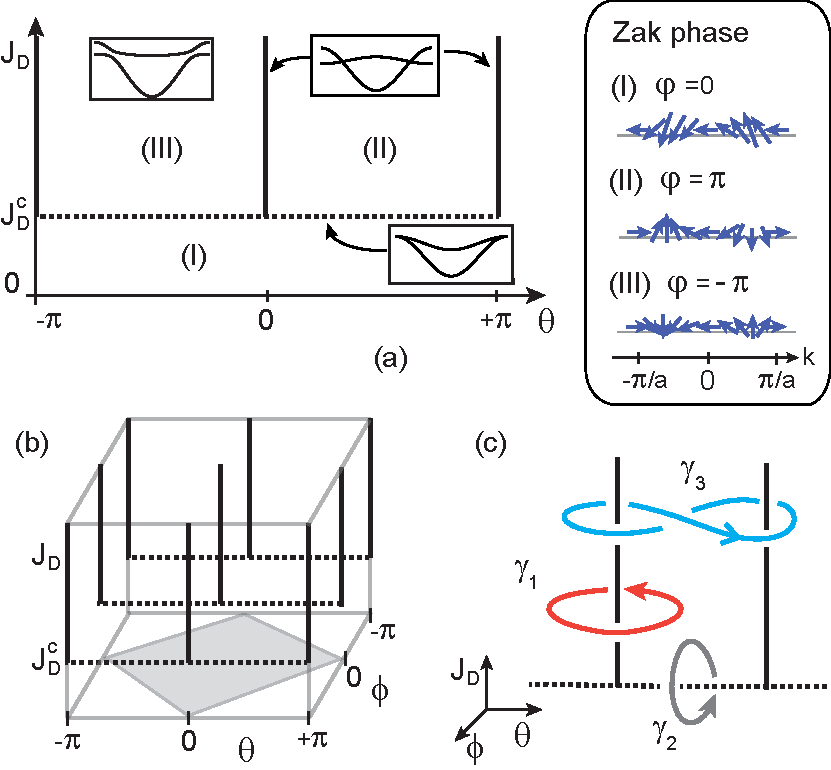
\includegraphics[width=1.\columnwidth]{creutz/fig2}
\caption{Creutz 模型完整拓扑相图。(a) 在 $\phi=0,\pm\pi$ 的平面内,$(J_D, \theta)$ 参数空间的拓扑相图,为 (b) 中之一截面;实线和虚线为相边界,都是体系发生简并的地方(因此也叫 degeneracy lines),在参数空间中穿过实线或虚线,体系发生能隙关闭再打开,并发生能带反转(band inversion);区别在于:实线上的点,能带有两个地方简并,将有两个能隙关闭再打开的情况,并且发生两次(同向的)band inversion,这也是模型中围绕其的非平庸周期演化路径能够发生内禀的以偶数单位拓扑电子输运的根源(见图\ref{fig:creutz:chargepumps});而虚线上的点,能带只有一个地方简并,发生一次能隙关闭再打开,一次能带反转,围绕其的非平庸路径就是上一节提到的 Rice-Mele 型拓扑电子输运;(a) 中的三幅插图标记了不同区域能带和能隙关闭的情况;(b) 模型在 $(J_D, \theta, \phi)$ 空间的完整的拓扑相图;(c) 围绕上述提到的两种 degeneracy lines 几种典型的周期含时演化环路:$\gamma_1$ 具有内禀为偶数单位的新奇拓扑输运,$\gamma_2$ 为普通单位为1的拓扑电子输运(Rice-Mele 型),$\gamma_3$ 为基于 $\gamma_1$ 人为构造的路径,具有单位为4的拓扑电子输运。右上角插图展示了 (a) 中几种情况下的 $Zak$ 相角\cite{creutz}。(取自\inlinecite{creutz})}
\label{fig:creutz:topophase}
\end{figure}

图中的实线和虚线代表不同的情况。在实线上,体系有两处地方发生简并
\footnote{见图 \ref{fig:creutz:topophase} (a) 右上插图。},
穿过其上的点将有两个能隙关闭再打开的行为,并且发生两个\textit{同向的}能带反转;而这也正是模型中围绕其的非平庸参数曲线的周期含时路径能够衍生出以偶数为单位的拓扑电子输运的原因,这种偶数单位的拓扑电子输运是内禀的行为,因为事实上绕其\textit{一}圈的参数曲线的电子输运 就为2,Chern 数为2,而绕其一圈已经是约化到最简的路径了,参见图 \ref{fig:creutz:topophase} (c) 中的 $\gamma_1$ 所示。
而在虚线上,体系仅有一处地方发生简并
\footnote{见图 \ref{fig:creutz:topophase} (a) 右下插图。},
穿过其上的点只有一个能隙关闭再打开的行为,只发生一次能带反转,因此围绕其路径 Chern 数为1,拓扑电子输运就是 以1为单位的Rice-Mele 型输运。

图 \ref{fig:creutz:topophase} (b) 给出了三维 $(J_D, \theta, \phi)$ 参数全空间的拓扑相图。图 \ref{fig:creutz:topophase} (a) 展示了其 $\phi=0,\pm\pi$ 时,$(J_D, \theta)$-平面内的情况,几个不同区间和相边界上的能带和能隙关闭情况在插图中给出。相应的,几个区域的 Zak 角在 图 \ref{fig:creutz:topophase} 右上角的插图中给出示意。图 \ref{fig:creutz:topophase} (c) 画出了几种典型的参数空间闭合环路的示意图,若使体系沿着这些环路具有含时依赖,将会发生拓扑电子输运的行为。其物理根源在上一节中有讨论。其中,$\gamma_1$ 环路的拓扑电子输运以2为单位的,$\gamma_2$ 的以1为单位,而 $\gamma_3$ 相当于两个 $\gamma_1$ 叠加,以 $4$ 为单位。
\footnote{注意,$\gamma_3$ 所绕的方向相反,但并没有抵消掉却是叠加上效果,原因是两条 degeneracy lines 发生的 band inversion 方向恰好相反。因此其相当于两个 $\gamma_1$ 叠加。}


\begin{figure}[!htb]
\centering
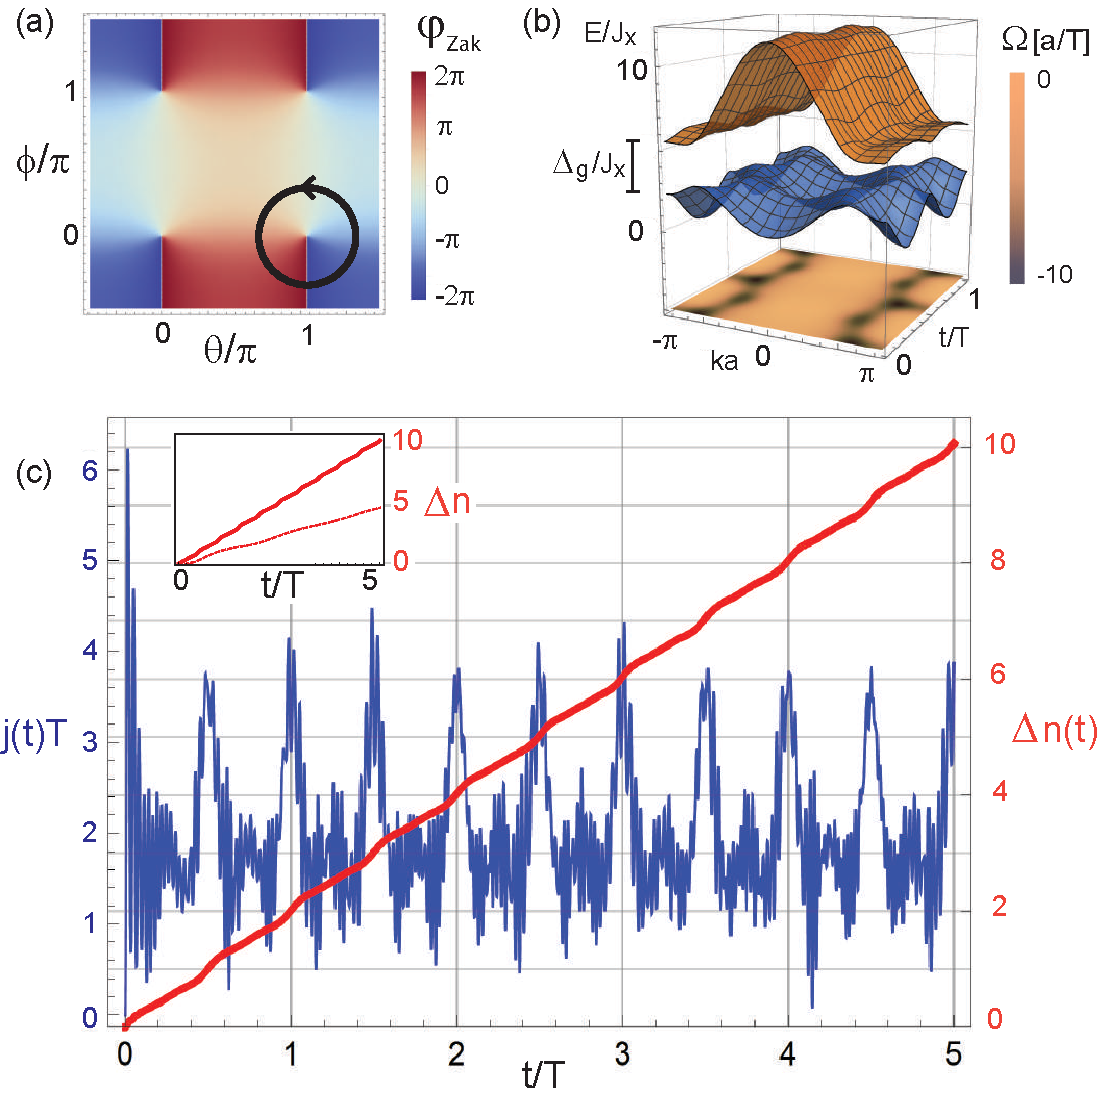
\includegraphics[width=1.\columnwidth]{creutz/fig3}
\caption{Creutz 模型中的拓扑电子输运过程。对于我们发现的内禀偶数为输运单位的新奇拓扑输运现象,我们进行了选取一个典型的路径进行了数值模拟的检验。(a) 含时演化的参数空间,$(\phi, \theta)$-平面,以及其上的Zak相角,黑色带箭头圆圈标记周期含时环路;(b) $(k,t)$ 参数空间的能带结构示意图(上),和基带的 Berry 曲率场(下); (c) 数值模拟含时薛定谔方程的演化的结果,蓝色曲线代表\textit{流}(current,$j(t)T$)的数值模拟结果(参照左侧蓝色纵坐标),红色曲线为电子输运(或Center-of-Mass,$\Delta n(t)$)的数值模拟结果(参照右侧红色纵坐标);电子输运为流的积分。可以看出,每个单位周期 $T$,体系输运 $2$ 单位的粒子,而且结果相当得量子化,肉眼可见的精度可以认定为整数。(c)中左上角的插图对比了在相同模型参数下,绝热演化(粗实线)和不绝热演化(细虚线)两种情况的电子输运,对比绝热条件下的高度量子化,非绝热条件下电子的输运不再量子化。这是由于非绝热的驱动下会将基带电子激发到高带。模型参数:$J_Y/J_X=2$, $J_D/J_X=1.8$, $\hbar\omega/J_x=0.1$(绝热情况),$6.0$(非绝热情况)。(取自\inlinecite{creutz})}
\label{fig:creutz:chargepumps}
\end{figure}

对于这种新奇的内禀输运单位为2的拓扑输运过程,我们选取一组典型的参数进行了数值计算。结果如图 \ref{fig:creutz:chargepumps} 所示。我们选取 $J_Y/J_X=2$, $J_D/J_X=1.8$,并选取图 \ref{fig:creutz:chargepumps} (a) 中所示的黑色带箭头环路作为闭合的周期性含时依赖路径,即
\begin{align}
\phi(t) &= \sin(\omega t) \\ 
\theta(t) &= \cos(\omega t)
\end{align}
其中 $\omega$ 为驱动频率,绝热条件要求 $\hbar\omega\ll J_X, J_Y, J_D$。在该组选定的参数下 $(\phi, \theta)$-平面内的 Zak 相角可以计算出来\cite{creutz},如图 \ref{fig:creutz:chargepumps} (a) 所示。对于现在该组参数下的含时模型,我们解析计算了其能带结构,如图 \ref{fig:creutz:chargepumps} (b) 上部所示。我们也计算了每个能带的 Berry 曲率场和 Chern 数,基带的 Berry 曲率场如图 \ref{fig:creutz:chargepumps} (b) 下部所示。这里用到了 Takahiro Fukui 等人在 2005 年的提出的二维材料的 Chern 数算法\inlinecite{chern2005},详见附录 \ref{sec:chern} 所述
\footnote{在附录 \ref{sec:chern} 中,我们详细讨论了该算法的性质,以及证明了相关的三个定理。这三个定理展示了该算法的有效性,以及量子化、规范不变等性质。我们还开发了分别基于 python3 语言 和 Wolfram Mathematica 语言的专门的程序包,开源地址见\inlinecite{repo-chern}。 }。 Chern 数为 Berry 曲率场的积分,该基带的 Chern 数为2。\footnote{对于这个简单的两能带模型,其 Chern 数本身很容易解析计算。数值方法作为一种检验,与解析方法结果吻合。}

Chern 数为2意味着该路径支持单位为2个电子的周期绝热拓扑电子输运过程。为检验,我们对该组参数下的绝热电子输运过程进行了数值模拟,驱动频率取作
\begin{align}
\hbar\omega/J_X = 0.1
\end{align}
通过数值模拟含时薛定谔方程的演化,我们计算出体系的\textit{流}($j$)和 电子输运($\Delta n$)随时间变化的值,如图 \ref{fig:creutz:chargepumps} (c) 所示。蓝色曲线表示流的值 $j(t)T$,参照左侧蓝色纵坐标;红色曲线表示电子输运的值 $\Delta n(t)$,参照右侧红色纵坐标。体系总的电子输运实为流的积分。
\begin{align}
\Delta n(t) = \int_0^t j(t')dt'
\end{align}

由图 \ref{fig:creutz:chargepumps} (c) 红色曲线可见,在 $\hbar\omega/J_X = 0.1$ 的频率驱动下,每个周期输运的电子为2,而且结果相当量子化,肉眼可见的精度内可以认定为整数。这说明,该频率下体系的演化已经相当绝热。作为对比,我们也计算了“不很绝热”的情况下的电子输运过程,取频率为
\begin{align}
\hbar\omega/J_X = 6.0
\end{align}
数值模拟结果图 \ref{fig:creutz:chargepumps} (c) 左上角插图中的细虚线。与绝热情况下的电子输运对比可见,此时的输运已不再量子化,单位周期输运不再具有为整数的量子化平台。该频率下前面提到的绝热条件将不被满足,存在从基带到高带的激发。





